\begin{frame}{Apprentissage}
	\begin{itemize}
		\item Les deux méthodes les plus communes
		\begin{itemize}
			\item Real Time Reccurent Learning (RTRL) \cite{Robinson87}
			\item BackPropagation Through Time (BPTT) \cite{Williams89}
		\end{itemize}
	\end{itemize}
\end{frame}

\begin{frame}{RTRL}

	\begin{itemize}
		\item On calcul l'erreur de gradient et on met à jour les poids à chaque pas
		\item  
	\end{itemize}
\end{frame}

\begin{frame}{BPTT 1/2}
	\begin{itemize}
		\item Déplier le réseau pour l'approximer par un réseau non récurrent 
		\item On applique une backprogation classique sur le réseau déplié
	\end{itemize}
    \begin{columns}
        \begin{column}{0.48\textwidth}
            \begin{figure}
                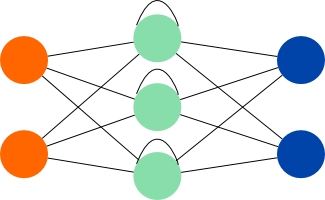
\includegraphics[width=.7\textwidth]{images/RNN_BPTT_ex}
                \caption{Exemple de RNN à l'instant t}
            \end{figure}
        \end{column}
        \begin{column}{0.48\textwidth}
            \begin{figure}
                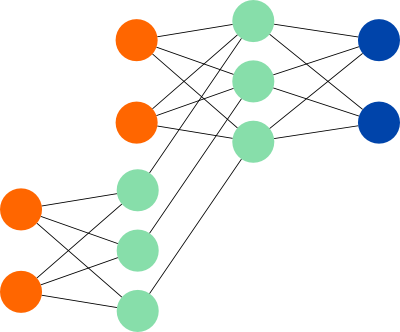
\includegraphics[width=.7\textwidth]{images/RNN_BPTT_dep_ex}
                \caption{RNN déplié jusqu'à l'instant t-1}
            \end{figure}
        \end{column}
    \end{columns}	
\end{frame}

\begin{frame}{BPTT 2/2}
	\begin{itemize}
		\item Défaut : Difficile d'utiliser cette méthode sur toute la période
		 \begin{itemize}
		 	\item On limite aux k dernières itérations : on oublie des informations
		 \end{itemize}
	\end{itemize}
\end{frame}